\chapter{Stand van zaken}
\label{ch:stand-van-zaken}

% Tip: Begin elk hoofdstuk met een paragraaf inleiding die beschrijft hoe
% dit hoofdstuk past binnen het geheel van de bachelorproef. Geef in het
% bijzonder aan wat de link is met het vorige en volgende hoofdstuk.

% Pas na deze inleidende paragraaf komt de eerste sectiehoofding.

%Dit hoofdstuk bevat je literatuurstudie. De inhoud gaat verder op de inleiding, maar zal het onderwerp van de bachelorproef *diepgaand* uitspitten. De bedoeling is dat de lezer na lezing van dit hoofdstuk helemaal op de hoogte is van de huidige stand van zaken (state-of-the-art) in het onderzoeksdomein. Iemand die niet vertrouwd is met het onderwerp, weet er nu voldoende om de rest van het verhaal te kunnen volgen, zonder dat die er nog andere informatie moet over opzoeken \autocite{Pollefliet2011}.
%
%Je verwijst bij elke bewering die je doet, vakterm die je introduceert, enz. naar je bronnen. In \LaTeX{} kan dat met het commando \texttt{$\backslash${textcite\{\}}} of \texttt{$\backslash${autocite\{\}}}. Als argument van het commando geef je de ``sleutel'' van een ``record'' in een bibliografische databank in het Bib\TeX{}-formaat (een tekstbestand). Als je expliciet naar de auteur verwijst in de zin, gebruik je \texttt{$\backslash${}textcite\{\}}.
%Soms wil je de auteur niet expliciet vernoemen, dan gebruik je \texttt{$\backslash${}autocite\{\}}. In de volgende paragraaf een voorbeeld van elk.
%
%\textcite{Knuth1998} schreef een van de standaardwerken over sorteer- en zoekalgoritmen. Experten zijn het erover eens dat cloud computing een interessante opportuniteit vormen, zowel voor gebruikers als voor dienstverleners op vlak van informatietechnologie~\autocite{Creeger2009}.

\section{Wat is Cloud Computing?}
 
 Cloud computing is alomtegenwoordig en een basiskennis van het begrip is interessant voor iedereen die werkt binnen de IT wereld. In dit hoofdstuk worden allerhande begrippen omtrent cloud computing geïntroduceerd. Na het lezen van dit hoofdstuk zal u in staat zijn om mee te praten over de basiscomponenten en workflows binnen cloud computing. De begrippen in dit hoofdstuk zijn van belang voor het vervolg van dit onderzoek naar serverless of FaaS. 

\subsection{Definitie}

Cloud computing is:
\newline
On-demand computing services die worden aangeboden via het internet. Deze services omvatten onder andere servers, databanken, netwerkfuncties, opslag en nog veel meer. Werken in de cloud volgt het principe: je betaalt voor wat je gebruikt. De cloud biedt flexibiliteit, schaalbaarheid en snelle provisioneer tijd. Het stelt bedrijven in staat benodigde IT infrastructuur uit te besteden en zo dus ook geld te besparen. In de cloud is het mogelijk om up- en down te schalen naargelang de huidige noden, de cloud is met andere woorden elastisch. \autocite{Davis2017}
\newline
\newline
Deze definitie vormt een algemene omschrijving van wat cloud computing allemaal kan inhouden. Het is enigszins zinvol om deze definitie te gebruiken als uitgangspunt om cloud computing verder in detail te omschrijven.

\subsection{Inleiding}
Afgelopen jaren is het internet en de wereld binnen IT enorm snel veranderd en geëvolueerd. Klassieke IT infrastructuur die werken volgens het client-server principe maken de transitie naar een cloudgebaseerde benadering. In een klassieke infrastructuur benadering koopt een bedrijf zelf servers aan, installeert en onderhoudt deze. Een bedrijf moet in dit opzicht alles voorzien: plaats, netwerk, elektriciteit, beveiliging, ... . Een eigen infrastructuur onderhouden in een opgezet datacenter brengt een grote kost met zich mee. In de beginjaren dat bedrijven hun datacenters opstelden werden er vaak voor alle applicaties aparte servers voorzien, met andere woorden er draaide toen één applicatie op één fysieke machine. De traditionele architectuur bracht grote kosten met zich mee en resulteerde vaak ook dat er op sommige momenten te veel resources waren in vergelijking met hoeveel men er maar nodig had. De klassieke benadering had dus heel wat beperkingen. 
\newline
\newline
Later introduceerde VMware als eerste een nieuw product: VMware Virtual Platform, virtualisatie was geboren. Virtualisatie zorgt ervoor dat bovenop de hardware van de server een ''Hypervisor'' kan worden geïnstalleerd. Een hypervisor is een programma dat toelaat om een server onder te verdelen in meerdere servers met elk hun eigen besturingssysteem. In de traditionele benadering werd er voor elke legacy-applicatie één server met één OS voorzien. Met gebruik van virtualisatie is het dus mogelijk om meerdere aparte servers te migreren naar één fysieke machine waarop een hypervisor draait. Het migreren van meerdere servers naar één fysieke machine zorgt ervoor dat de resources beter benut worden. Dankzij de hypersvisor draaien meerdere servers nog steeds onafhankelijk van elkaar op hun eigen besturingssysteem op dezelfde fysieke hardware. Virtualisatie zorgt ervoor dat er minder fysieke servers  moeten worden aangekocht wat de kost dus aanzienlijk vermindert. Binnen virtualisatie kunnen ook complexe netwerken worden gebouwd zodat gevirtualiseerde servers met elkaar en de buitenwereld kunnen communiceren. \autocite{RedHat2019}. In 
figuur ~\ref{fig:klassiek-vs-virtualisatie} wordt het verschil tussen een klassieke server met één OS en één applicatie vergeleken met een server waarop gevirtualiseerde servers draaien. Virtualisatie ligt aan de fundamenten van cloud computing, deze technologie maakt het vandaag de dag mogelijk om infrastructuur te draaien in de cloud.
\newline
\newline
\begin{figure}
    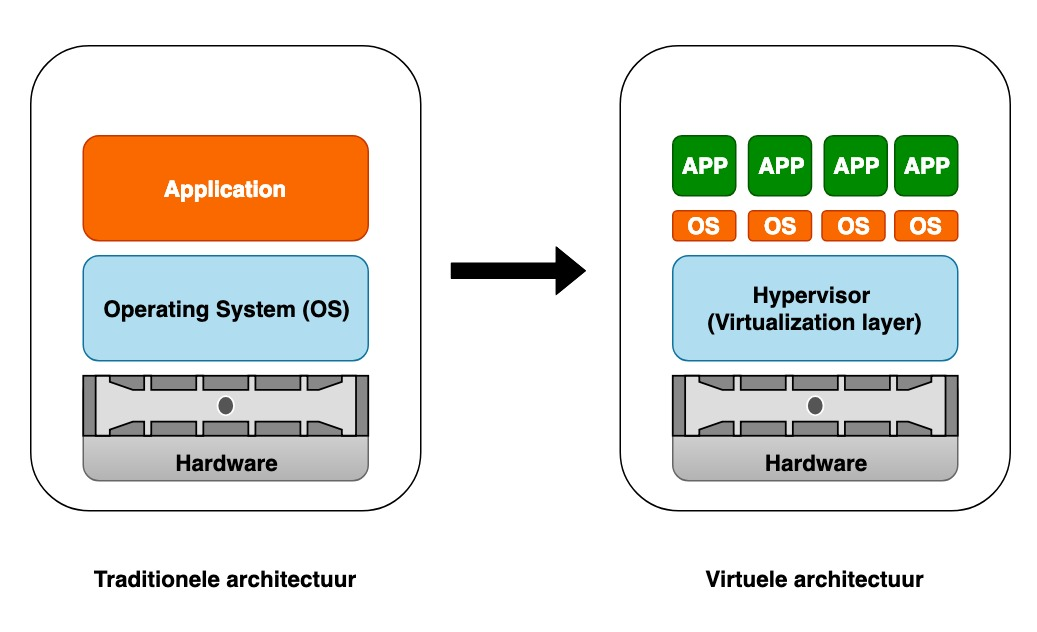
\includegraphics[width=1\textwidth]{img/klassiek_virtualisatie}
    \caption{De architectuur aan de linkerkant weergeeft een beeld van hoe de traditionele server architectuur eruit zag. De afbeelding rechts toont hoe een gevirtualiseerde architectuur eruitziet.} 
    \label{fig:klassiek-vs-virtualisatie}  
\end{figure}
\newline

Wanneer er naar de cloud gerefereerd wordt, dan bedoelt men meestal de cloud services die grote providers als een Google, Amazon en Microsoft aanbieden. Laten we de conventie maken dat wanneer er in de inleiding gerefereerd wordt naar de cloud, dat dit wijst op de cloud services die door cloud providers worden aangeboden. Later maken we de distinctie tussen welke verschillende soorten cloud er zijn met elk hun eigenschappen. De afgelopen jaren hebben steeds meer bedrijven gekozen om hun applicaties en infrastructuur naar de cloud te migreren. Migratie naar de cloud is interessant in verschillende opzichten, er zijn heel wat voordelen aan verbonden die in sectie ~\ref{voor-en-nadelen} worden uitgelegd. De grootste motivatie waarom bedrijven naar de cloud migreren is enerzijds het feit dat er enkel betaald wordt voor wat men verbruikt en anderzijds neemt het heel wat overhead zoals het onderhouden van infrastructuur weg. Cloud computing zorgt ervoor dat gebruikers een gedeelde poel van resources en opslag kunnen gebruiken bij een cloud provider, deze poel kan worden gezien als duizenden servers waarop virtuele machines of applicaties die worden aangeboden kunnen worden gedraaid. Deze services worden verschaft via het internet. Gebruikers betalen enkel voor de resources die ze verbruiken, zo worden de kosten meestal berekend op de tijd die een server draait en welke gespecificeerde resources deze verbruikt, zo een model wordt ook wel het ''Pay as you go model'' genoemd . De cloud is veelzijdig en biedt mogelijkheden op verschillende niveaus, deze worden in volgende onderdelen besproken.\autocite{Seghal2018} 


\subsection{Cloud types op deployment niveau}
\label{cloud-deployment-level}
De Cloud kan worden onderverdeeld in verschillende types op niveau van deployment. De onderverdeling op deployment level slaat op de locatie waar de cloud infrastructuur draait, bijvoorbeeld in een datacenter van een grote cloud provider of bij een bedrijf op locatie in een eigen datacenter. Volgens \textcite{Goyal2014} kan de cloud worden opgedeeld in vier verschillende soorten met elk hun specifieke eigenschappen. Om te beginnen wordt ook besproken wat men bedoelt met on-premises infrastructuur.

\subsubsection{On-premises}
Een on-premises infrastructuur wijst op een IT infrastructuur die wordt beheerd door een organisatie zelf, de apparaten bevinden zich ook op locatie bij het bedrijf. Een organisatie die over een on-premises of op locatie infrastructuur beschikt staat in voor het volledige beheer hiervan, dit gaat van fysieke installatie van apparaten netwerk enzovoort tot het beveiligen van applicatie op niveau van software. Een on-premises installatie zien we vaak terug in klassieke benaderingen of in bedrijven waar ze nog niet overtuigd van het hele cloud gebeuren. Sommige organisaties kiezen expliciet om hun infrastructuur niet in de cloud te draaien om allerhande redenen gerelateerd aan privacy en confidentialiteit van data.

\subsubsection{Publieke cloud}
De publieke Cloud wordt onderhouden door een derde partij. Publieke cloud providers bieden services en resources aan die op basis van een soort huurcontract aan externen worden verschaft. Klanten die services of infrastructuur huren bij publieke cloud providers kunnen deze raadplegen via het internet. Publieke cloud services worden verschaft aan iedereen, ze zijn met andere woorden voor iedereen toegankelijk. De publieke cloud stelt organisaties in staat te besparen op aankoop van infrastructuur. Het is mogelijk om te betalen naargelang de resources of diensten die worden gebruikt en dit is een heel interessant aspect van de publieke cloud. Data die gemaakt of opgeslagen wordt door gebruikers bevindt zich ook in het datacenter van de cloud provider. Voorbeelden van publieke cloud providers zijn, zoals eerder al aangehaald, Google, Amazon en Microsoft.

\subsubsection{Private cloud}
Private cloud bestaat in verschillende opzichten, het kan een datacenter zijn dat op locatie staat en onderhouden wordt of een cloud infrastructuur zijn die is opgezet in een datacenter waar servers worden gehuurd. Een private cloud wordt door de organisatie zelf volledig onderhouden, er is ook enkel toegang voor de organisatie zelf of voor toegestane derde partijen. Wanneer er gekozen wordt voor een private cloud infrastructuur dan brengt dit de veelzijdigheid en tools van cloud computing met zich mee, het is mogelijk dezelfde tools uit de publieke cloud op te zetten in een private cloudomgeving. Private cloud wordt vooral gekozen voor het waarborgen van privacy en veiligheid van data. Deze benadering wordt door veel bedrijven gekozen die veel confidentiële- en bedrijfskritische data moeten verwerken, denk maar aan banken, overheid en farmaceutica.

\subsubsection{Hybride cloud}
Een hybride cloud bestaat uit minstens één private en één publieke cloud. Wanneer verschillende soorten cloud met elkaar worden samengebracht wordt er verwezen naar een hybride cloud. Een hybride cloud wordt opgezet volgens verschillende standaarden en cloud- en apparatuur specifieke patenten. Een hybride cloud biedt de veelzijdigheid voor up- en down schaling zoals in de publieke cloud, en de veiligheid en integriteit zoals in de private cloud. Het implementeren van een hybride cloud omgeving is moeilijker omdat security hier heel wat overhead met zich meebrengt.

\subsubsection{Communtiy cloud}
Community cloud valt tussen de publieke en private cloud. Een community cloud bestaat uit twee of meer deelnemende partijen. Dit type van cloud valt te vergelijken met de private cloud die gedeeld wordt door meerdere partijen. Gebruik van een community cloud reduceert de aankoopkost van infrastructuur en de management kosten voor het opzetten van het cloud datacenter.


\subsection{Cloud service modellen}
\label{cloud-service-level}
Naast onderscheid op basis van de locatie waar cloud infrastructuur gedeployed wordt, maakt men ook onderscheid op niveau van service. Termen zoals PaaS, IaaS en SaaS horen tot deze sectie \autocite{Goyal2014}, in volgende drie secties worden deze veelvoorkomende klassieke cloud computing modellen samengevat.

\subsubsection{Infrastructure-as-a-Service (IaaS)}
Het IaaS service model biedt gebruikers computing, processing, networking en opslag aan waarop applicaties en dergelijke kunnen worden gedraaid. De gebruiker heeft de mogelijkheid om bovenop hardware die voorzien wordt door de cloud provider in te staan voor het volledige beheer van de infrastructuur. De componenten die aanpasbaar zijn, zijn onder andere het OS, de middleware, runtime, data en applicaties. De cloud provider staat in voor de networking, opslag, fysieke servers en bovenliggende virtualisatie. IaaS vormt de basis waarop Cloud computing is gebouwd, overige service modellen bouwen hierop ook verder. Gebruikers die controle willen hebben over (bijna) alle onderdelen van hun cloud infrastructuur opteren voor het gebruik van IaaS. Voorbeelden van IaaS zijn onder andere Google Cloud Platform Compute Engine, Amazon Web Services EC2 en Microsoft Azure.

\subsubsection{Platform-as-a-Service (PaaS)}
PaaS is vooral gericht op ontwikkelaars. Platform-as-a-Service stelt gebruikers in staat op een eenvoudige manier softwareapplicaties op te zetten zonder zorgen over de onderliggende infrastructuur. Cloud providers die PaaS diensten verschaffen staan in voor het volledige beheer van de infrastructuur zoals servers, zowel virtueel als fysiek, computing, opslag, netwerk, beveiliging, bijhorende tools en API's. Het beheer van servers zoals OS en dergelijke wordt ook door de cloud provider voorzien, PaaS voorziet een platform om applicaties op te draaien. Gebruikers staan enkel in voor ontwikkeling van de applicatie en de data die daar bijhoort. Als PaaS oplossing wordt vaak AWS Elastic Beanstalk gebruikt.

\subsubsection{Software-as-a-Service (SaaS)}
In het Software-as-a-Service model wordt de gehele infrastructuur inclusief applicatie beheerd door de provider. SaaS voorziet applicaties die draaien in de cloud en raadpleegbaar zijn via een computer of mobiel apparaat, vaak simpelweg via een webbrowser. In het verleden moest software meestal worden aangekocht en worden geïnstalleerd op individuelen systemen, SaaS is hiervoor de oplossing. Wanneer er gebruik wordt gemaakt van SaaS wordt de software aangerekend ob basis van subscripties per gebruiker, dit kan op basis van tijd of verbruik. SaaS draait, zoals eerder gezegd, in de cloud en vereist dus geen extra installatie van software. Eén van de bekendste SaaS applicaties is Office 365, deze Microsoft services werken met een maandelijkse subscriptie die betaald wordt per gebruiker. Een voorbeeld van een gratis SaaS applicatie is bijvoorbeeld Google Docs.
\begin{figure}
    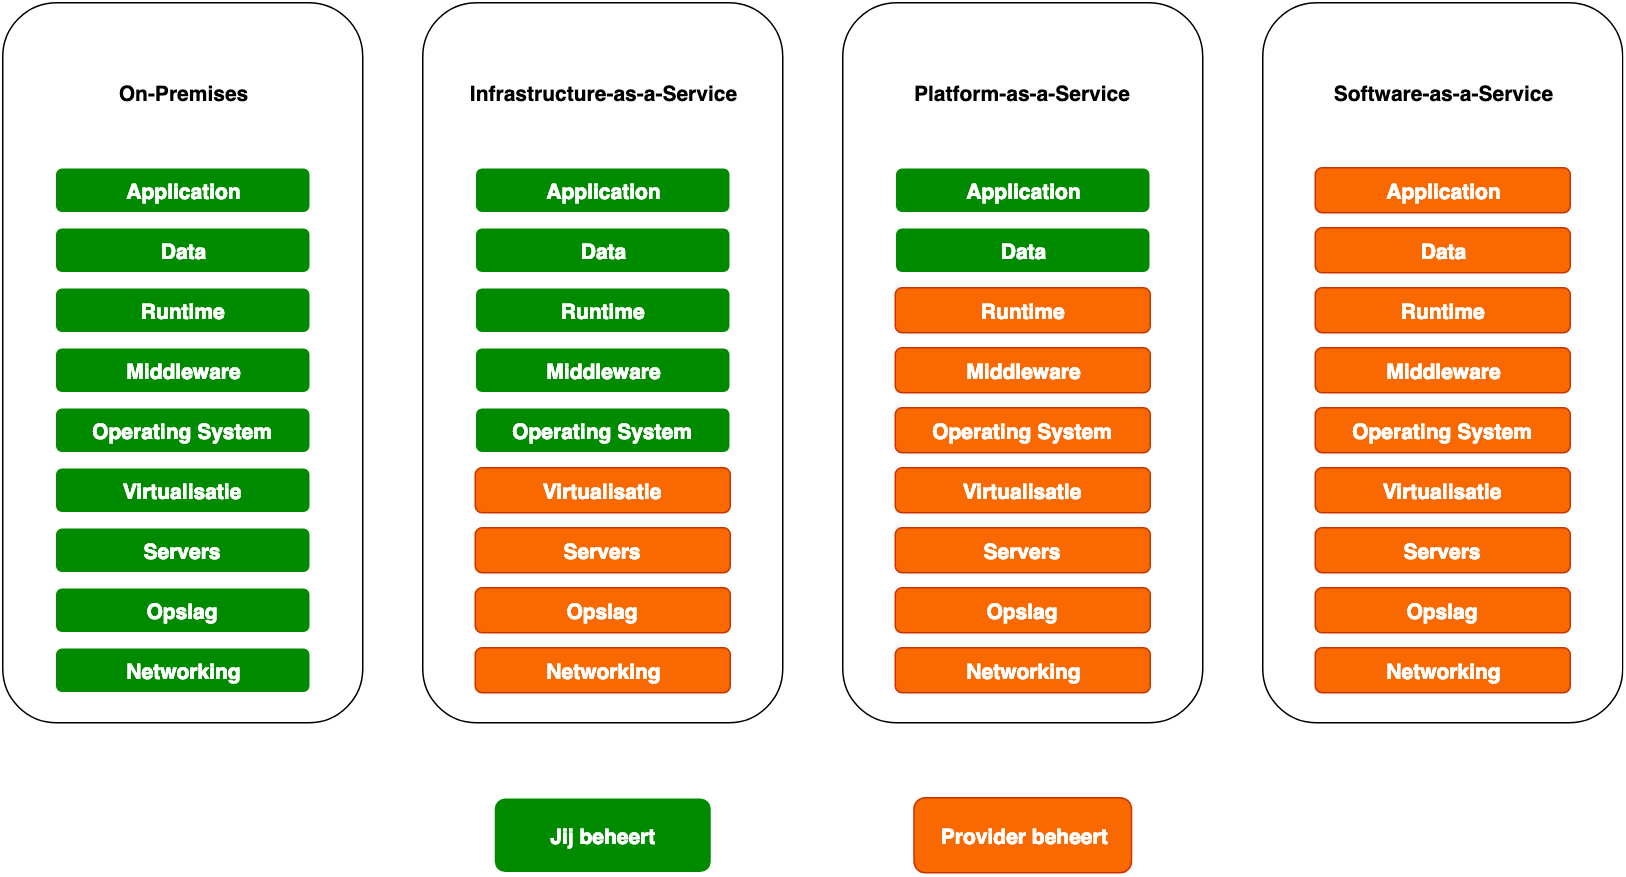
\includegraphics[width=1\textwidth]{img/cloud_service_level.png}
    \caption{De afbeelding weergeeft een schematische voorstelling van de verschillende cloud service niveaus. De groene kleur duidt alle onderdelen aan die zelf te managen zijn. De oranje kleur geeft aan welke onderdelen de cloud provider beheert.} 
    \label{fig:cloud-service-levels}  
\end{figure}
\newline

\subsection{Voor-en nadelen}
\label{voor-en-nadelen}
Cloud computing kent voordelen die heel wat mogelijkheden bieden ten opzichte van de klassieke benadering omtrent infrastructuur. \autocite{Azure2019} De voordelen zijn veelbelovend maar ook de nadelen mogen zeker niet over het hoofd worden gezien en dienen in kaart te worden gebracht om op de hoogte te zijn van mogelijke gevaren en bedreigingen.\autocite{Sosinsky2011} 

\subsubsection{Voordelen}

\begin{description}[style=unboxed, labelwidth=\linewidth, listparindent =0pt]
    \item[Lagere kosten]
    Cloud computing zorgt ervoor dat bedrijven zelf geen fysieke hardware meer hoeven aan te kopen voor hun eigen datacenter om software en applicaties te draaien. Een bedrijf hoeft bijvoorbeeld zelf geen webserver meer aan te kopen en te installeren om een webapplicatie te kunnen draaien, de benodigde hardware is beschikbaar bij verschillende cloud providers. Daarnaast zijn er ook geen kosten voor elektriciteitsvoorzieningen. De enige kost zijn de prijzen die de cloud provider aanrekent om de apparatuur of diensten ter beschikking te stellen.
    \newline

    \item[Performantie]
    Datacenters van grote cloud providers bevinden zich verspreid doorheen de hele wereld. De verspreiding van datacenters zorgt voor een lage latency en zorgt ervoor dat werken in de cloud voelt alsof de server in het eigen bedrijf staat. Computing componenten worden ook geregeld geüpgrade naar de laatste versies zodat de performantie verzekerd kan worden.
    \newline

    \item [Veiligheid]
    Doordat servers en opslag niet meer op locatie staan bij bedrijven wordt de kans op datadiefstal al sterk gereduceerd. Er is geen fysieke toegang meer tot infrastructuur en dus zal het onmogelijk zijn om via deze weg data te stelen. Daarnaast zijn datacenters uitgerust met dedicated beveiligingsapparatuur die in vele bedrijven niet aanwezig is. Datacenters zelf zijn erg goed beveiligd, het is haast onmogelijk deze gebouwen te betreden. Op softwareniveau bieden cloud providers ook heel wat diensten aan die helpen bij het beveiligen van applicaties.
    \newline

    \item [Schaalbaarheid en flexibiliteit]
    Cloud computing stelt in staat om up- en down te schalen volgens de noden. Dit wilt zeggen dat een bedrijf eender wanneer kan opteren om meer of minder middelen te huren naar gelang wat nodig is. Cloud computing is met andere woorden elastisch. Een bedrijf zoals Tomorrowland kan bijvoorbeeld doorheen het jaar, wanneer er geen ticketverkoop aan de gang is, de requests naar hun webservers bolwerken met 10 operationele servers. Indien er een ticketverkoop start kan het bedrijf kiezen om op te schalen naar 300 webservers zodat alle requests kunnen worden behandelt zonder dat dit veel moeite kost. De nood voor 30 keer meer servers is, wanneer deze manueel worden geïnstalleerd en opgezet op locatie, een taak die heel veel tijd en werk in beslag neemt maar die in de cloud zo is verwerkt. Dit voorbeeld toont aan dat de cloud mogelijkheden biedt om op een eenvoudige manier te schalen zonder dat dit handenvol geld kost (infrastructuur, tijd).
    \newline
  
\end{description}

\subsubsection{Nadelen}


\begin{description}[style=unboxed, labelwidth=\linewidth, listparindent =0pt]
        \item[Latency]
        Wanneer datacenters ver liggen vanwaar de servers worden geraadpleegd. Bijvoorbeeld je gebruikt thuis, in België, een applicatie die draait in een datacenter in de Verenigde staten, dan kan er latency optreden. Latency is vertraging in datacommunicatie tussen twee systemen, ook wel bekend als ''lag''. Dit probleem begint stilaan te verdwijnen aangezien alle grote cloud providers datacenters verdeeld hebben over de hele wereld.
        \newline
        
        \item[Privacy en security]
        Data legt meestal een langere weg af tussen een klant en cloud provider wanneer er gebruik wordt gemaakt van cloud services dan wanneer die klant zelf gebruik maakt van een infrastructuur op locatie. De langere route die de data neemt brengt ook meer gevaar met zich mee, hoe verder data moet reizen, hoe meer kans op onderschepping. Daarnaast is er vaak geen garantie of de overheid niet meekijkt naar de data die zich in datacenters bevindt bij publieke cloud providers. Datacenters zijn voor hackers ook grote doelwitten omdat ze met mogelijke inbraken hier veel mensen mee kunnen treffen en gegevens kunnen stelen.
        \newline
        
        \item [Vendor lock-in]
        Wanneer er gekozen wordt om gebruik te maken van diensten die een bepaalde cloud provider aanbiedt dan zit je vast aan die cloud provider en is overstappen met je hele infrastructuur vaak een zware klus. Kiezen om over te stappen naar een andere provider brengt mogelijks heel wat complexiteit en problemen met zich mee.
        \newline
        
        
        \item [Afhankelijk van netwerkconnectiviteit]
        Bij gebruik van de publieke cloud is er steeds afhankelijkheid van netwerkconnectiviteit. Wanneer een internetverbinding niet mogelijk is door eventuele problemen bij de Internet Service Provider (ISP) dan kan de cloud niet bereikt worden en zorgt dit voor grote problemen wanneer een bedrijf afhankelijk is van alles wat in de cloud draait. Daarnaast is het ook van belang dat er een snelle netwerkverbinding met voldoende bandbreedte beschikbaar is om effectief en efficiënt gebruik te maken van de cloud.
        \newline
        
        \item [Downtime]
        Downtime is een nadeel dat nog voor problemen kan zorgen. Wanneer een infrastructuur gedraaid wordt binnen een bepaald datacenter en dit gaat neer door interne problemen (technische problemen, onderhoud, gefaalde update/upgrade, brand, natuurramp, ...) dan zijn de infrastructuur en diensten (tijdelijk) niet meer bereikbaar. In het allerslechtste geval kunnen zo ook alle gegevens verloren raken wanneer er geen failover voorzien werd naar een ander datacenter (bijvoorbeeld in geval van een natuurramp). De kans dat dit voorkomt is echter nihil.
\end{description}
\newpage

\section{Wat is Serverless?}
Sinds de geboorte van de cloud hebben cloud diensten en technologieën een enorme (re)volutie gekend, denk maar aan de brede waaier van diensten die grote cloud providers vandaag aanbieden. Serverless  is ook een technologie die nog maar enkele jaren wordt aangeboden door cloud providers. Velen hebben waarschijnlijk wel al eens over de term ''Serverless'' gehoord maar weten vaak niet wat het inhoudt. Serverless wordt vaak omschreven als de volgende evolutie in cloud computing, een die van gelijkaardig succes kan zijn als het succes van zijn voorgangers zoals IaaS, PaaS en SaaS. Serverless brengt heel wat begrippen met zich mee, deze worden allemaal behandelt in volgende secties.
 
\subsection{Definitie}
De termen serverless en FaaS worden vaak door elkaar gebruikt en deze verwijzen dan vaak naar het volledige serverless plaatje, toch betekenen ze beiden niet hetzelfde. Wanneer er gesproken wordt over serverless computing dan kan er een onderscheid worden gemaakt in twee onderdelen met elk zijn eigen specifieke eigenschappen. Enerzijds is er Backend-as-a-Service (BaaS) en anderzijds Function-as-a-Service (FaaS). Het onderscheid dat wordt gemaakt tussen beiden duidt ook meteen dat serverless meer is dan enkel FaaS en dat de term serverless en FaaS daarom niet als synoniemen gebruikt zouden mogen worden. Echter in de praktijk wanneer men spreekt over serverless, dan bedoelt men meestal altijd de FaaS benadering. Het vervolg van dit onderzoek richt zich ook op Function-as-a-Service. De bijhorende proof-of-concept is ook gebaseerd op Faas.\autocite{Roberts2017}

\subsubsection{Backend-as-a-Service (BaaS)}
Backend-as-a-Service stelt ontwikkelaars in staat om gebruik te maken van kant en klare oplossingen zodat ze zelf geen server-side of backend componenten meer hoeven te managen. BaaS is een cloud service model dat verantwoordelijk is voor het volledige management van  de backend van een applicatie. Ontwikkelaars kunnen het beheer van backend servers outsourcen aan aanbieders van Backend-as-a-Service, dit stelt hun in staat te focussen op hetgeen dat er voor hen wel toe doet namelijk de applicatie code, de frontend. Waar het op neer komt is dat BaaS applicaties opsplitst in meerdere kleine onderdelen, deze opsplitsing zorgt ervoor dat verschillende ontwikkelaars gebruik kunnen maken van dezelfde delen software die reeds eerder zijn geschreven en worden aangeboden door een Backend-as-a-Service vendor. Wat dit betekend is dat ontwikkelaars dus gebruik kunnen maken van bestaande modules en deze implementeren in de backend van hun applicatie, denk bijvoorbeeld aan een database achterliggend aan een applicatie, integratie met sociale media of een module voor gebruikersauthenticatie zoals Auth0. BaaS providers zoals Google's Firebase biedt bijvoorbeeld een database aan die in de backend wordt onderhouden en aangeboden door de BaaS providers zonder dat de ontwikkelaar zich moet focussen op dit backend component. Daarnaast bieden BaaS providers nog een waaier van andere diensten aan om het leven van een ontwikkelaar zo aangenaam mogelijk te maken.
\\
De server-side mogelijkheden die de meeste Backend-as-a-Service providers aanbieden zijn:
\begin{itemize}
    \item Hosting van de applicatie, het beheer van de servers waarop de applicatie draait
    \item Opslag in de cloud voor content die gegenereerd wordt door gebruikers
    \item Management van een achterliggende databank
    \item Push notificaties
    \item Authenticatie voor gebruikers
    \item Beheer van updates
\end{itemize}
BaaS is vooral terug te vinden in de ontwikkeling van mobiele applicaties, er wordt ook vaak naar gerefereerd als Mobile-Backend-as-a-service (MBaaS). Backend-as-a-Service wordt gezien als serverless benadering omdat de ontwikkelaar enkel nog focust op de code die hij schrijft en niet op de servers waarop deze code draait. Serverless of zonder servers betekend dus niet dat er geen servers zijn, maar gewoon dat een ontwikkelaar zich er geen zorgen meer hoeft over te maken. BaaS brengt een groot nadeel met zich mee en dat is de vendor lock-in. Wanneer een ontwikkelaar kiest voor diensten bij een bepaalde vendor, dan is het moeilijk om in latere stadia weg te gaan bij die vendor.\autocite{Cloudflare2019} 

\subsubsection{Function as a Service (FaaS)}
Wanneer er gesproken wordt over serverless dan bedoelt men meestal de Function-as-a-Service cloud service en niet de Backend-as-a-Service benadering.  Function-as-a-Service is een trend in softwareontwikkeling die gebaseerd is op het schrijven en deployen van verschillende individuele functies.  
\\
In het deployment van klassieke applicaties wordt een applicatie traditioneel gedraaid in een virtuele machine (VM) of in een container. Wanneer de host een container of een VM is, dan draait de applicatie als proces bovenop op het besturingssysteem. De achterliggende code van een applicatie bevat vaak verschillende, aan elkaar gerelateerde, methoden met elk hun eigen functionaliteit.  Figuur \ref{fig:traditional-software-deployment} geeft een visualisatie van klassieke software deployment benadering, er is duidelijk te zien dat binnen een host de applicatie draait als een proces met daarbinnen de individuele methoden die elkaar aanspreken om de functionaliteit van de applicatie te garanderen.
\begin{figure}
    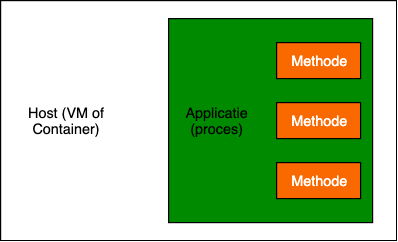
\includegraphics[width=0.7\textwidth]{img/traditional_software_deployment.png}
    \caption{Klassieke monoliet applicaties draaien als één proces op een besturingssysteem binnen een container of virtuele machine. Ee klassieke applicatie is opgebouwd uit verschillende methoden met elk hun eigen functionaliteit gescheiden door softwareklassen.} 
    \label{fig:traditional-software-deployment}  
\end{figure}
\\
De FaaS benadering verandert het klassieke model van applicatie deployment. Ontwikkelaars schrijven in dit model individuele functies die losstaan van elkaar en elk hun eigen specifieke taak hebben. Een applicatie draait nu niet meer voortdurend in een VM of container maar de functionaliteit werkt event-driven. De functies die de ontwikkelaar schrijf worden opgeladen naar een FaaS platform. Omdat de applicatie niet meer voortdurend draait is het FaaS platform zo geconfigureerd dat het luistert naar events die gekoppeld zijn aan een specifieke functie. Wanneer er een event optreedt dat een functie aanroept dan zorgt het FaaS platform ervoor dat er een container op wordt gebracht, de code wordt ingeladen en uitgevoerd en na afloop van de functie wordt de container weer gestopt. Functies worden vaak aangeroepen aan de hand van HTTP API Gateway calls, in de voorbeelden die volgen wordt de cyclus van FaaS duidelijk weergegeven. Hoe dit nu serverless is? Wel , ontwikkelaars dienen zich enkel maar te focussen op het schrijven van code (functies) en deze plaatsen ze gewoon in het FaaS platform, de achterliggende infrastructuur daar hoeven ze zich niets van aan te trekken.\autocite{Roberts2017}
\\\\
Er zijn al heel wat cloud providers die Function-as-a-Service platforms aanbieden en de populairste op moment van schrijven zijn ongetwijfeld: Amazon Web Services met hun AWS Lambda, Google Cloud Platform met Google Cloud Functions en Microsoft Azure met Azure Functions. De opgesomde platformen zijn allen proprietary en dus niet open-source. De FaaS platformen die de grote spelers aanbieden zijn al ver ontwikkeld en bieden heel wat functionaliteit maar zullen niet verder behandelt worden in dit onderzoek. Als alternatief duiken er steeds meer en meer open-source frameworks op voor het opzetten van een FaaS platform. In verder onderzoek zal een overweging worden gemaakt welke twee open-source frameworks het meest interessant zijn voor Nubera, die aan hun vereisten voldoen.

\section{Serverless concepten, begrippen en onderdelen}
Wat serverless nu precies voorstelt zou na het lezen van de definities al een stuk duidelijker moeten zijn. Serverless brengt echter nog meer begrippen mee om het volledige plaatje te kunnen schetsen. In deze sectie worden de belangrijkste ''key concepts'' met bijhorende begrippen nader verklaard.

\subsubsection{Next-Gen applicaties}
Naar applicaties die draaien in een serverless omgeving wordt vaak gerefereerd als next-gen applicaties. Met next-generation applicaties bedoelen we de applicaties die in een Cloud gebaseerde omgeving draaien en een onderliggende architectuur hebben die bestaat uit enerzijds containers en anderzijds microservices. Applicatieontwikkeling is de afgelopen jaren enorm veranderd, nu is het hele development gebeuren gericht op continue integratie en continue delivery (CI/CD) en zijn de ontwikkelingscyclussen (tijd tussen applicatie releases) verkleind van een aantal weken of aantal maanden tot een aantal minuten, uren of weken in het slechtste geval. 

\subsubsection{Microservices}
Microservices is een alternatief voor klassieke monoliet applicaties, dit zijn applicaties die verschillende functionaliteiten omvatten en draaien als een enkel proces binnen een VM of container. Een monoliet applicatie kan worden gezien als één gehele applicatie die draait op één machine.  In microservices daarentegen worden verschillende functionaliteiten en services gegroepeerd in groepen met elk hun eigen verantwoordelijkheden. Microservices zijn als het ware  een decompositie van een monoliet applicatie. Applicaties ontwikkeld volgens een microservices architectuur bestaan uit onafhankelijke componenten die naast elkaar bestaan en makkelijk vervangbaar of upgradebaar zijn. In een klassiek ontwerp van een applicatie is de applicatielogica van elkaar gescheiden door behulp van verschillende softwareklassen, deze kunnen met elkaar communiceren. In een microservice architectuur kunnen de verschillende componenten ook met elkaar communiceren maar dit gebeurt aan de hand van REST API vaak via het HTTP protocol. Daar waar monoliet applicaties gebruik maken van eenzelfde datastore, zijn elk component van microservices verantwoordelijk voor hun eigen data en persistentie. Een microservice kan de data van een andere microservice niet rechtstreeks raadplegen. Verschillende microservices kunnen draaien in verschillende VMs of containers, daarom wordt deze architectuur ook wel loosely-coupled genoemd.\autocite{Fowler2014}

\subsubsection{Containers}
In essentie is een container te vergelijken met een zeer kleine VM. Volgens \textcite{Docker2019} is een container een stuk software dat alle code en dependencies van een applicatie omvat zodat een applicatie op eender welke computeromgeving hetzelfde draait. De container bevat alles dat een applicatie nodig heeft om te kunnen werken naar behoren, onder andere: code, runtime, systeem programma's zoals binaries, systeem libraries en instellingen. Een ontwikkelaar is in staat om zelf container samen te stellen die voldoet aan zijn/haar vereisten. Concreet kan een ontwikkelaar dus een container image maken en hieruit kan dan een container worden opgezet. Een container image en de container die daaruit wordt opgebouwd ziet er overal hetzelfde uit ongeacht het onderliggend systeem. Figuur \ref{fig:virtualisatie_vs_containers} toont het verschil in architectuur tussen een gevirtualiseerde infrastructuur en een infrastructuur waarin containers draaien.
 \begin{figure}
     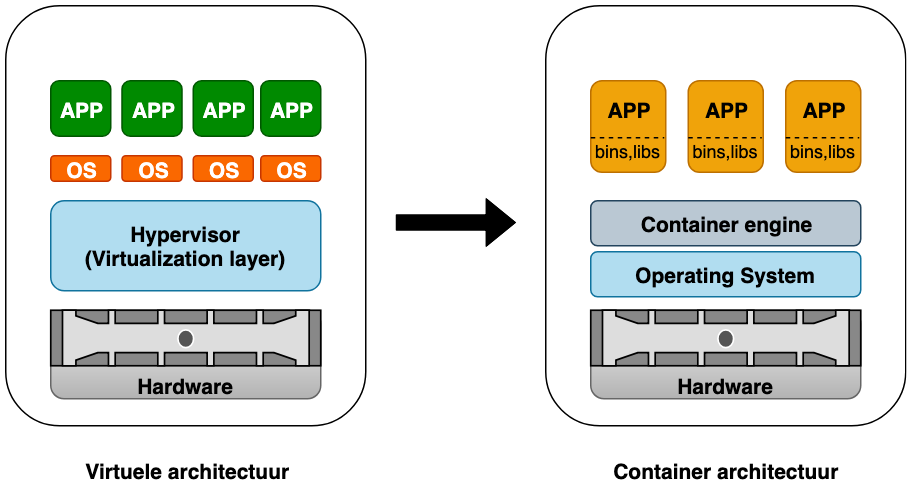
\includegraphics[width=1\textwidth]{img/virtualisatie_vs_containers.png}
     \caption{De figuur links geeft een representatie van een gevirtualiseerde architectuur. Rechts is er een gecontaineriseerde architectuur te zien. Bovenop de hardware en het besturingssysteem draait een container engine, de bekendste container engine is ongetwijfeld Docker engine. Bovenop de container enigne draaien de containers met elk hun eigen binaries, libraries en applicatie.} 
     \label{fig:virtualisatie_vs_containers}  
 \end{figure}


\subsubsection{API Gateway}
Wanneer functies worden aangeroepen, dan gebeurt dat binnen FaaS vaak via een API gateway aan de hand van HTTP. Microservices communiceren ook met elkaar via deze API gateways, op die manier kunnen verschillende microservices gebruik maken van elkaars functionaliteit.
\textcite{Roberts2017} beschrijven de taak van een API gateways als die van een webserver die verantwoordelijk is voor het ontvangen en routeren van HTTP requests. Een request dat wordt ontvangen wordt gerouteerd naar de handler gebaseerd op de route van de HTTP request. De API gateway ontvangt het antwoord van de handler en routeert dit uiteindelijk terug naar de originele client. Zoals eerder al aangehaald zijn handlers binnen FaaS infrastructuren vaak de functies geschreven door de ontwikkelaars. De API gateway is op de hoogte van alle handlers waar requests naar kunnen worden gerouteerd, deze worden meegegeven in de configuratie van de API. Figuur \ref{fig:api-gateway} geeft een schematische voorstelling van hoe een API gateway eruitziet.
 
 \begin{figure}
    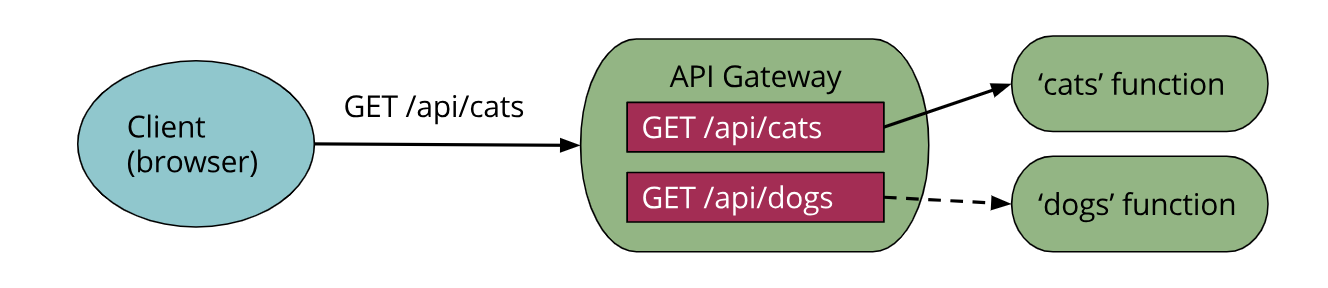
\includegraphics[width=1\textwidth]{img/api_gateway.png}
    \caption{In de figuur is een schematische voorstelling van het API gateway concept te zien. Wanneer een client (webbrowser) een HTTP GET request verstuurd naar het pad /api/cats, dan ontvangt de API gateway dit request en zoekt in zijn configuratie de overeenkomstige handler. Wanneer de handler is gevonden wordt het GET request doorgestuurd naar de handler, in dit geval een functie genaamd ''cats''. De functie retourneert de opgevraagde inhoud naar de API gateway die het request op zijn beurt terugstuurt naar de originele client, in dit geval de webbrowser.\autocite{Roberts2018}} 
    \label{fig:api-gateway}  
\end{figure}

\section{Serverless architectuur}
Hoe serverless infrastructuren eruitzien wordt in deze sectie uitgelegd aan de hand van voorbeelden gebaseerd op een zeer interessant artikel over serverless computing door \textcite{Roberts2018}.
\subsubsection{Applicaties met een user-interface}
In dit voorbeeld bestaat de architectuur uit de klassieke drie-lagen benadering. Er is een client systeem, in dit geval een webbrowser, een server met serverlogica en applicatiecode en een achterliggende databank voor persistentie. De benadering die hier gehanteerd wordt zorgt ervoor dat de client van niets op de hoogte is en dat alle logica aanwezig is in het systeem. De applicatieserver is verantwoordelijk voor alle functionaliteiten zoals: authenticatie, navigatie, zoekmogelijkheden en transacties. In figuur \ref{fig:drielagen_architectuur} wordt de architectuur schematisch voorgesteld.
\begin{figure}
    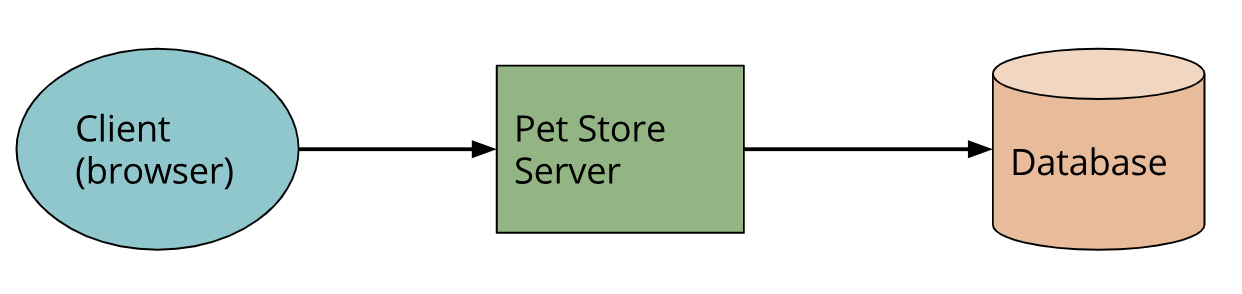
\includegraphics[width=1\textwidth]{img/drielagen_architectuur.png}
    \caption{De figuur weergeeft een schematische voorstelling van een klassieke applicatie opgebouwd volgens het drie-lagen model. De client fungeert enkel als grafische interface en bevat niets van achterliggende code. De applicatieserver bevat alle applicatielogica en maakt gebruik van een achterliggend databanksysteem. \autocite{Roberts2018}} 
    \label{fig:drielagen_architectuur}  
\end{figure}
\\\\
Wanneer de klassieke benadering wordt omgevormd volgens een serverless architectuur, dan wordt de applicatie op een volledig andere manier ontwikkeld zodanig dat nu ook de client verantwoordelijkheden heeft en alles niet afhankelijk is van één enkele applicatieserver. Figuur \ref{fig:serverless_architectuur} geeft een overzicht van de opbouw van de applicatie in een serverless omgeving.
\begin{figure}
    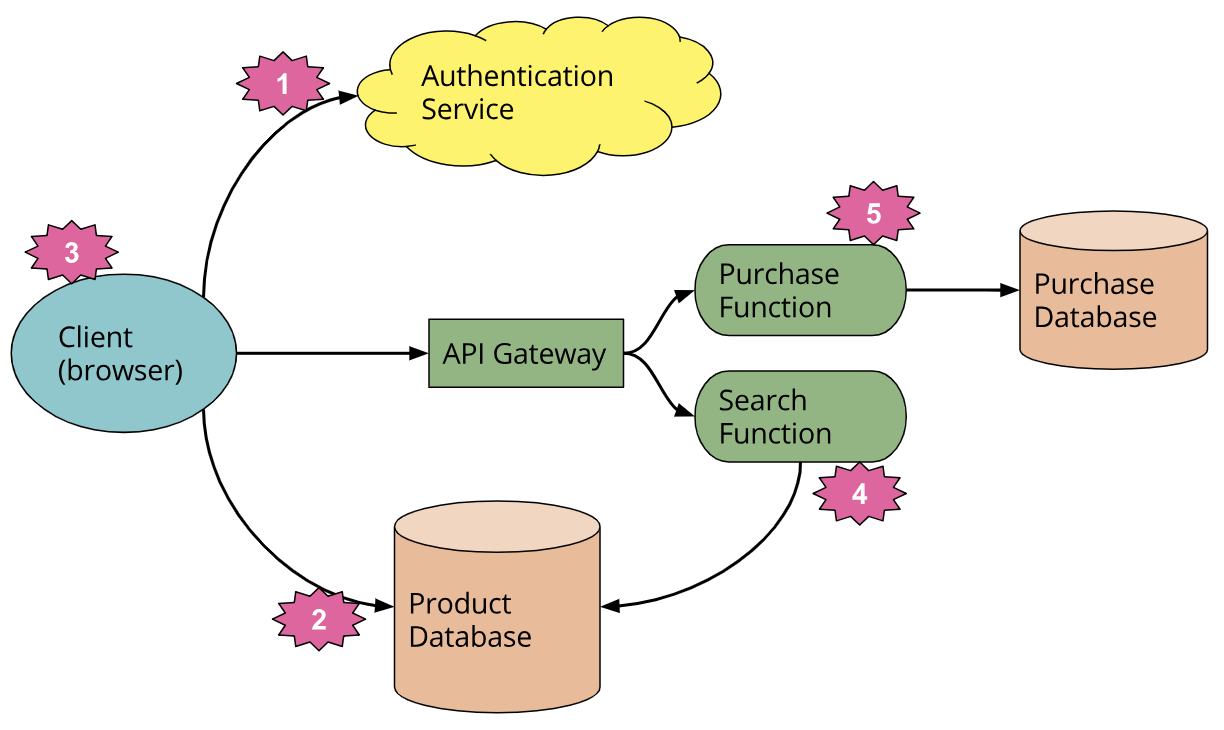
\includegraphics[width=1\textwidth]{img/serverless_architectuur.png}
    \caption{De figuur weergeeft een schematische voorstelling van een applicatie die opgebouwd is volgens een serverless architectuur. De applicatielogica wordt nu opgesplitst in verschillende microservices met elk hun eigen functionaliteit. \autocite{Roberts2018}} 
    \label{fig:serverless_architectuur}  
\end{figure}
In de figuur zijn onmiddellijk enkele grote verschillen te bemerken in vergelijking met de klassieke drie-lagen architectuur zoals in figuur \ref{fig:drielagen_architectuur}:
\begin{enumerate}
    \item De authenticatie logica die initieel verwerkt was in de applicatie op de applicatieserver is verplaatst uit de applicatie en wordt vervangen door een Backend-as-a-Service dienst die wordt aangeboden door een derde partij, bijvoorbeeld Okta.
    \item De databank die eerst enkel raadpleegbaar was door de applicatieserver is nu ook te bereiken door de client. De databank wordt uitbesteed aan een derde partij alweer als BaaS dienst, een mogelijkheid hiervoor is Google Firebase zoals eerder in dit onderzoek al werd aangehaald.
\end{enumerate}